\documentclass{article}
\usepackage[T2A]{fontenc}
\usepackage[utf8]{inputenc}
\usepackage[english, russian]{babel}
\usepackage{minted}
\usepackage{graphicx}
\usepackage{caption}



\newenvironment{pseudolisting}
 {\begin{minipage}{\linewidth}\vspace*{\topsep}}
 {\vspace*{\topsep}\end{minipage}}

\begin{document}

\begin{titlepage}
  \begin{center}
    \large
     
    \textbf{Федеральное государственное автономное образовательное учреждение высшего образования}
    \vspace{0.5cm}
 
    НАЦИОНАЛЬНЫЙ ИССЛЕДОВАТЕЛЬСКИЙ УНИВЕРСИТЕТ \\ "ВЫСШАЯ ШКОЛА ЭКОНОМИКИ"
    \vspace{0.5cm}
     
    Московский институт электроники и математики имени А. Н. Тихонова 
     
    Программа "Прикладная математика"
    \vfill
     
     
    Нигматуллин Роман Максимович
    \vfill
 
    \textsc{Лаборатная работа}\\[5mm]
     
    {\LARGE Теория погрешностей и машинная арифметика\\[2mm]
    }
  \bigskip
     
    3 курс, группа БПМ203
\end{center}
\vfill
 

 
\hfill\begin{flushright}
  \textbf{Преподаватель:}\\
  Брандышев Петр Евгеньевич
\end{flushright}%
\vfill
 
\begin{center}
  Москва, 2021 г.
\end{center}
\end{titlepage}

\section{Расчет частичных сумм ряда}

\begin{pseudolisting}
\inputminted{python}{series.py}
\end{pseudolisting}

\newpage
\begin{center}
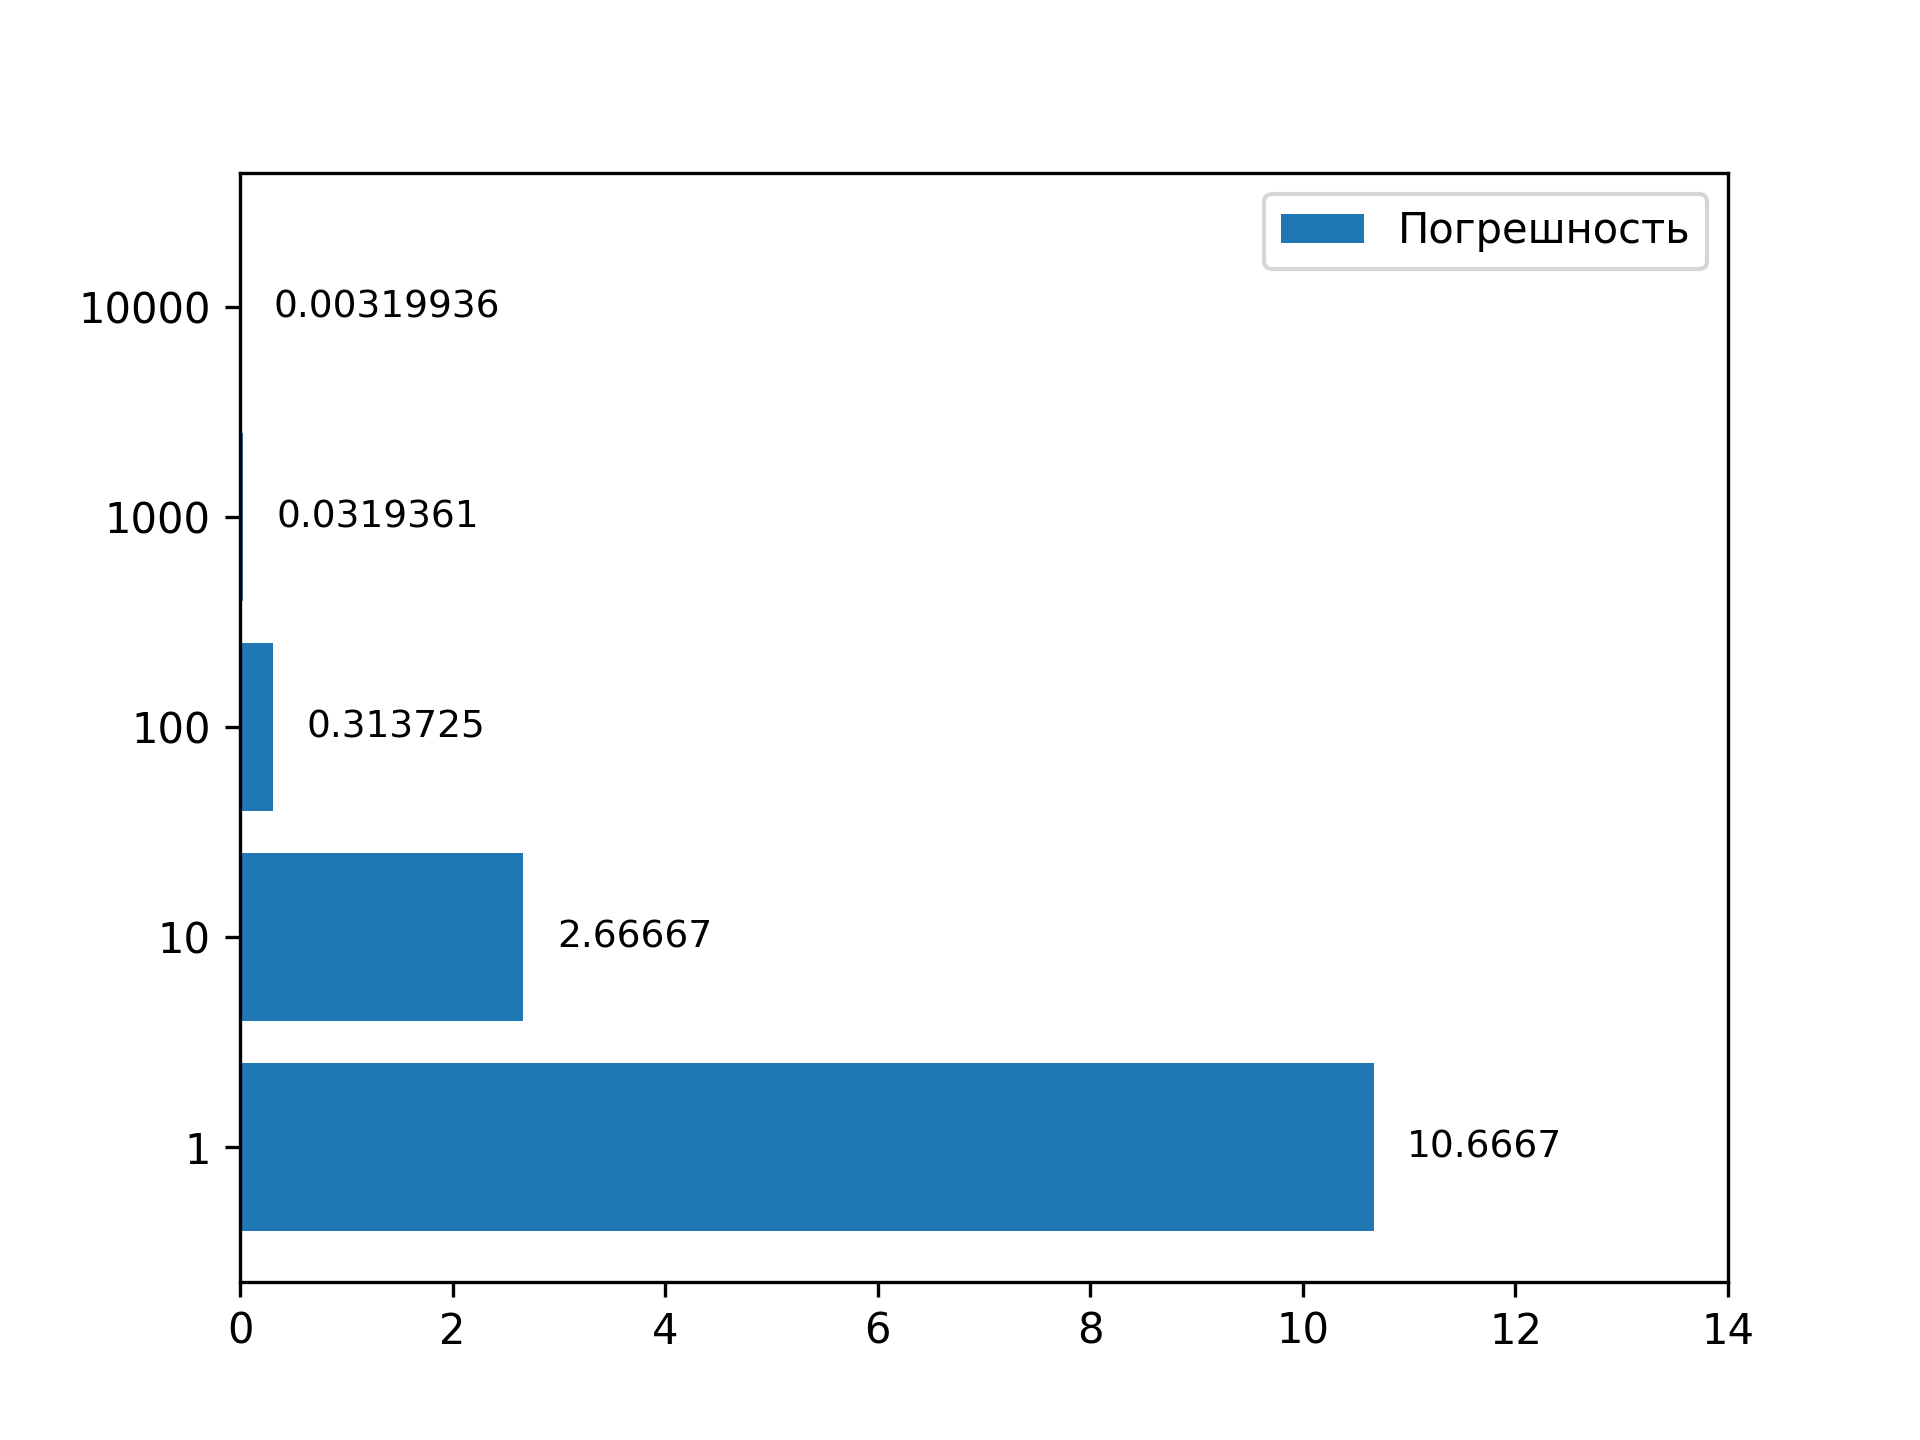
\includegraphics[width=\textwidth]{plots/series_error.png}
\end{center}
\begin{center}
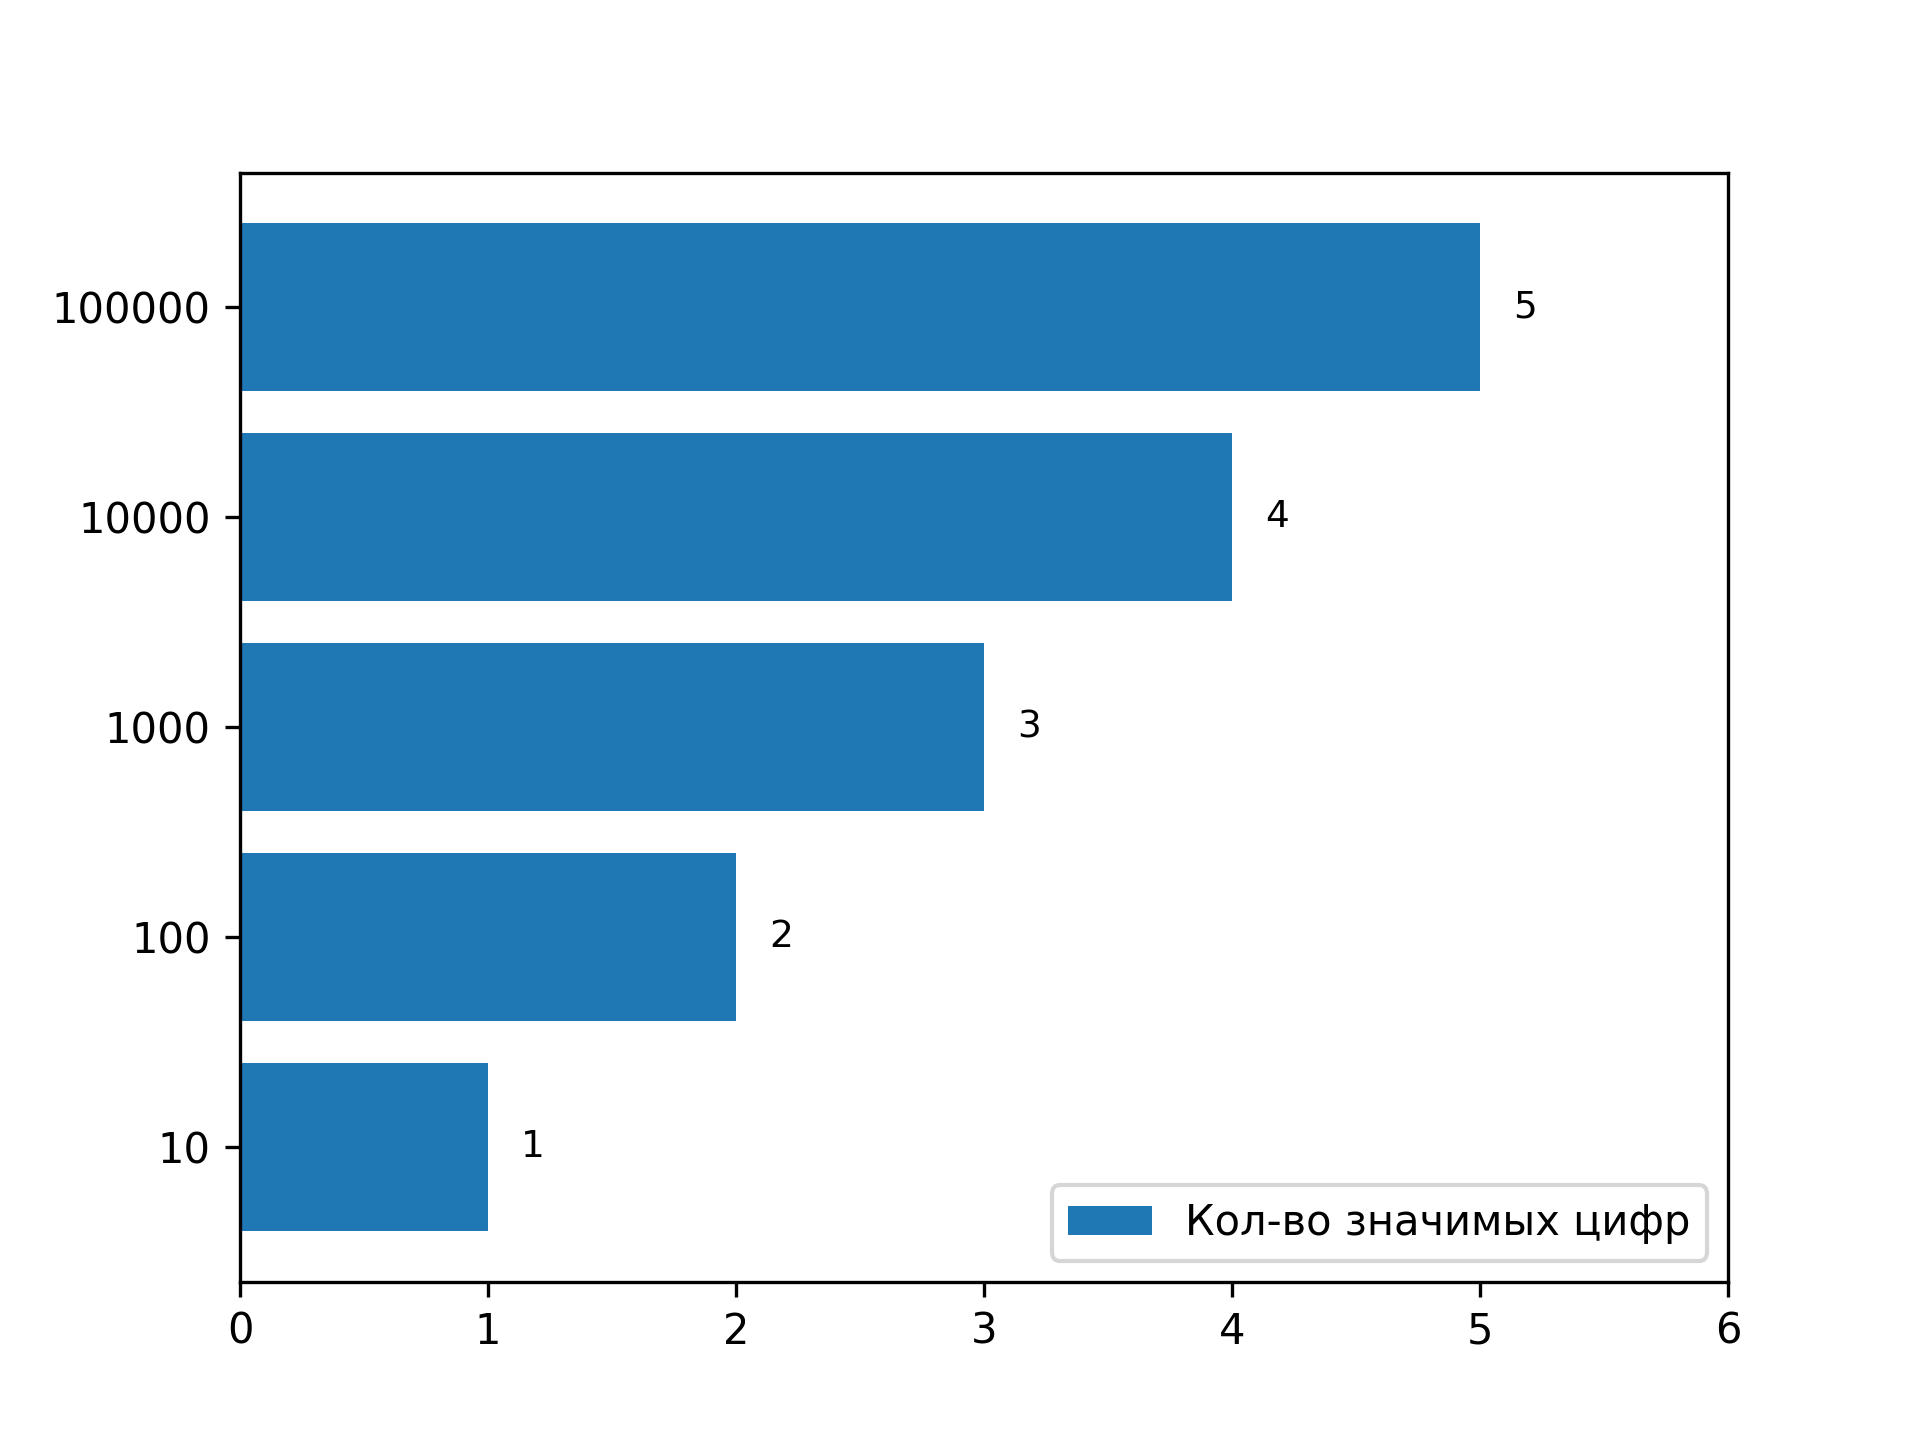
\includegraphics[width=\textwidth]{plots/series_n_digits.png}
\end{center}
\section{Вычисления с ограниченной разрядностью}

\begin{center}
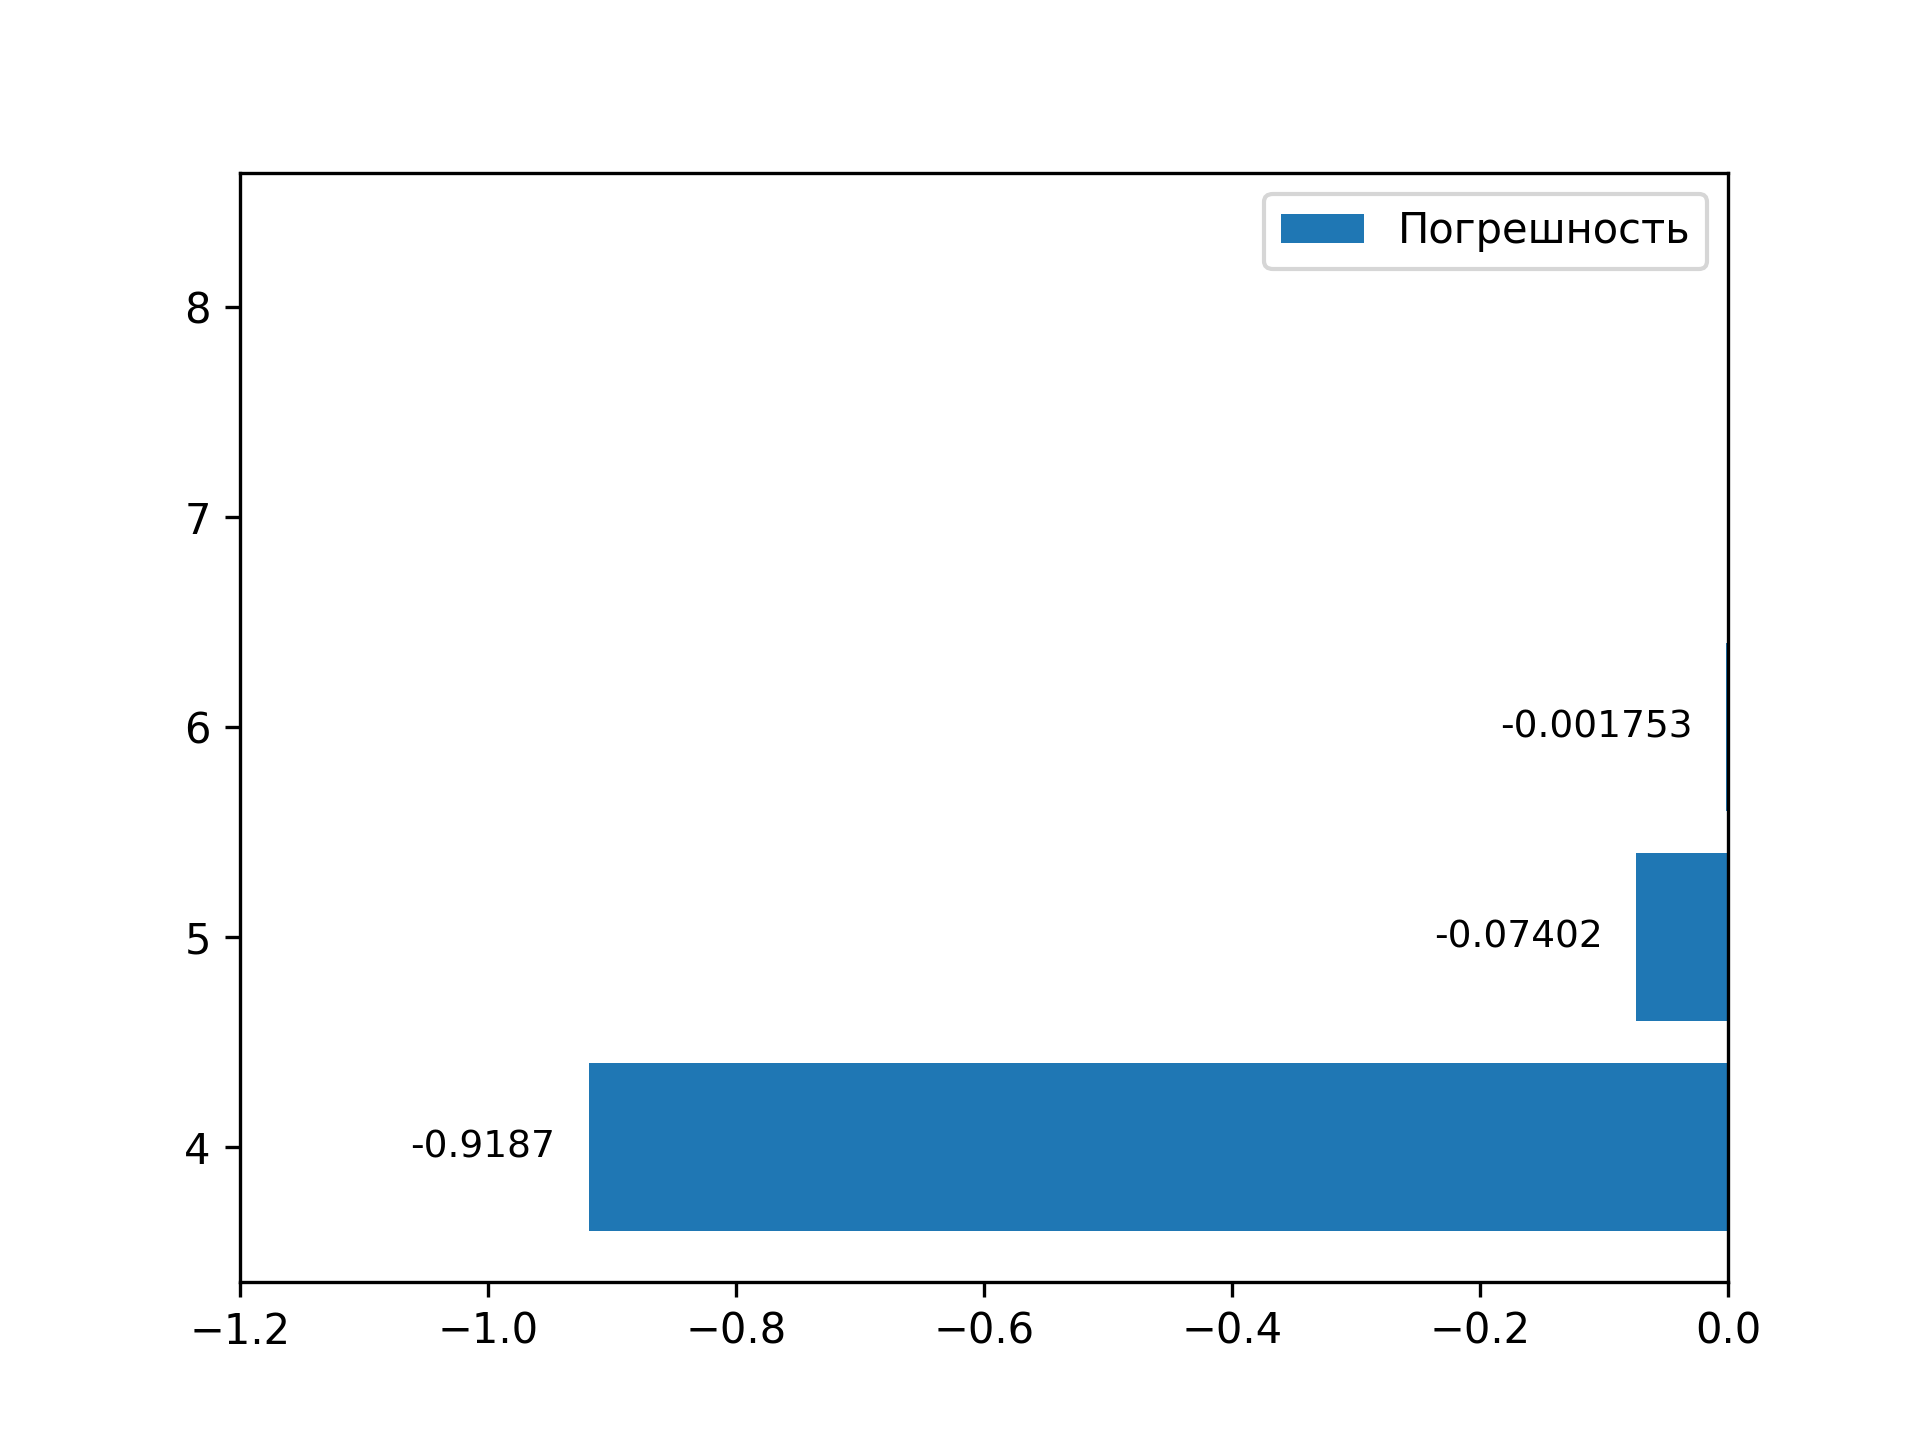
\includegraphics[width=\textwidth]{plots/series_fixed_error.png}
\end{center}
\begin{center}
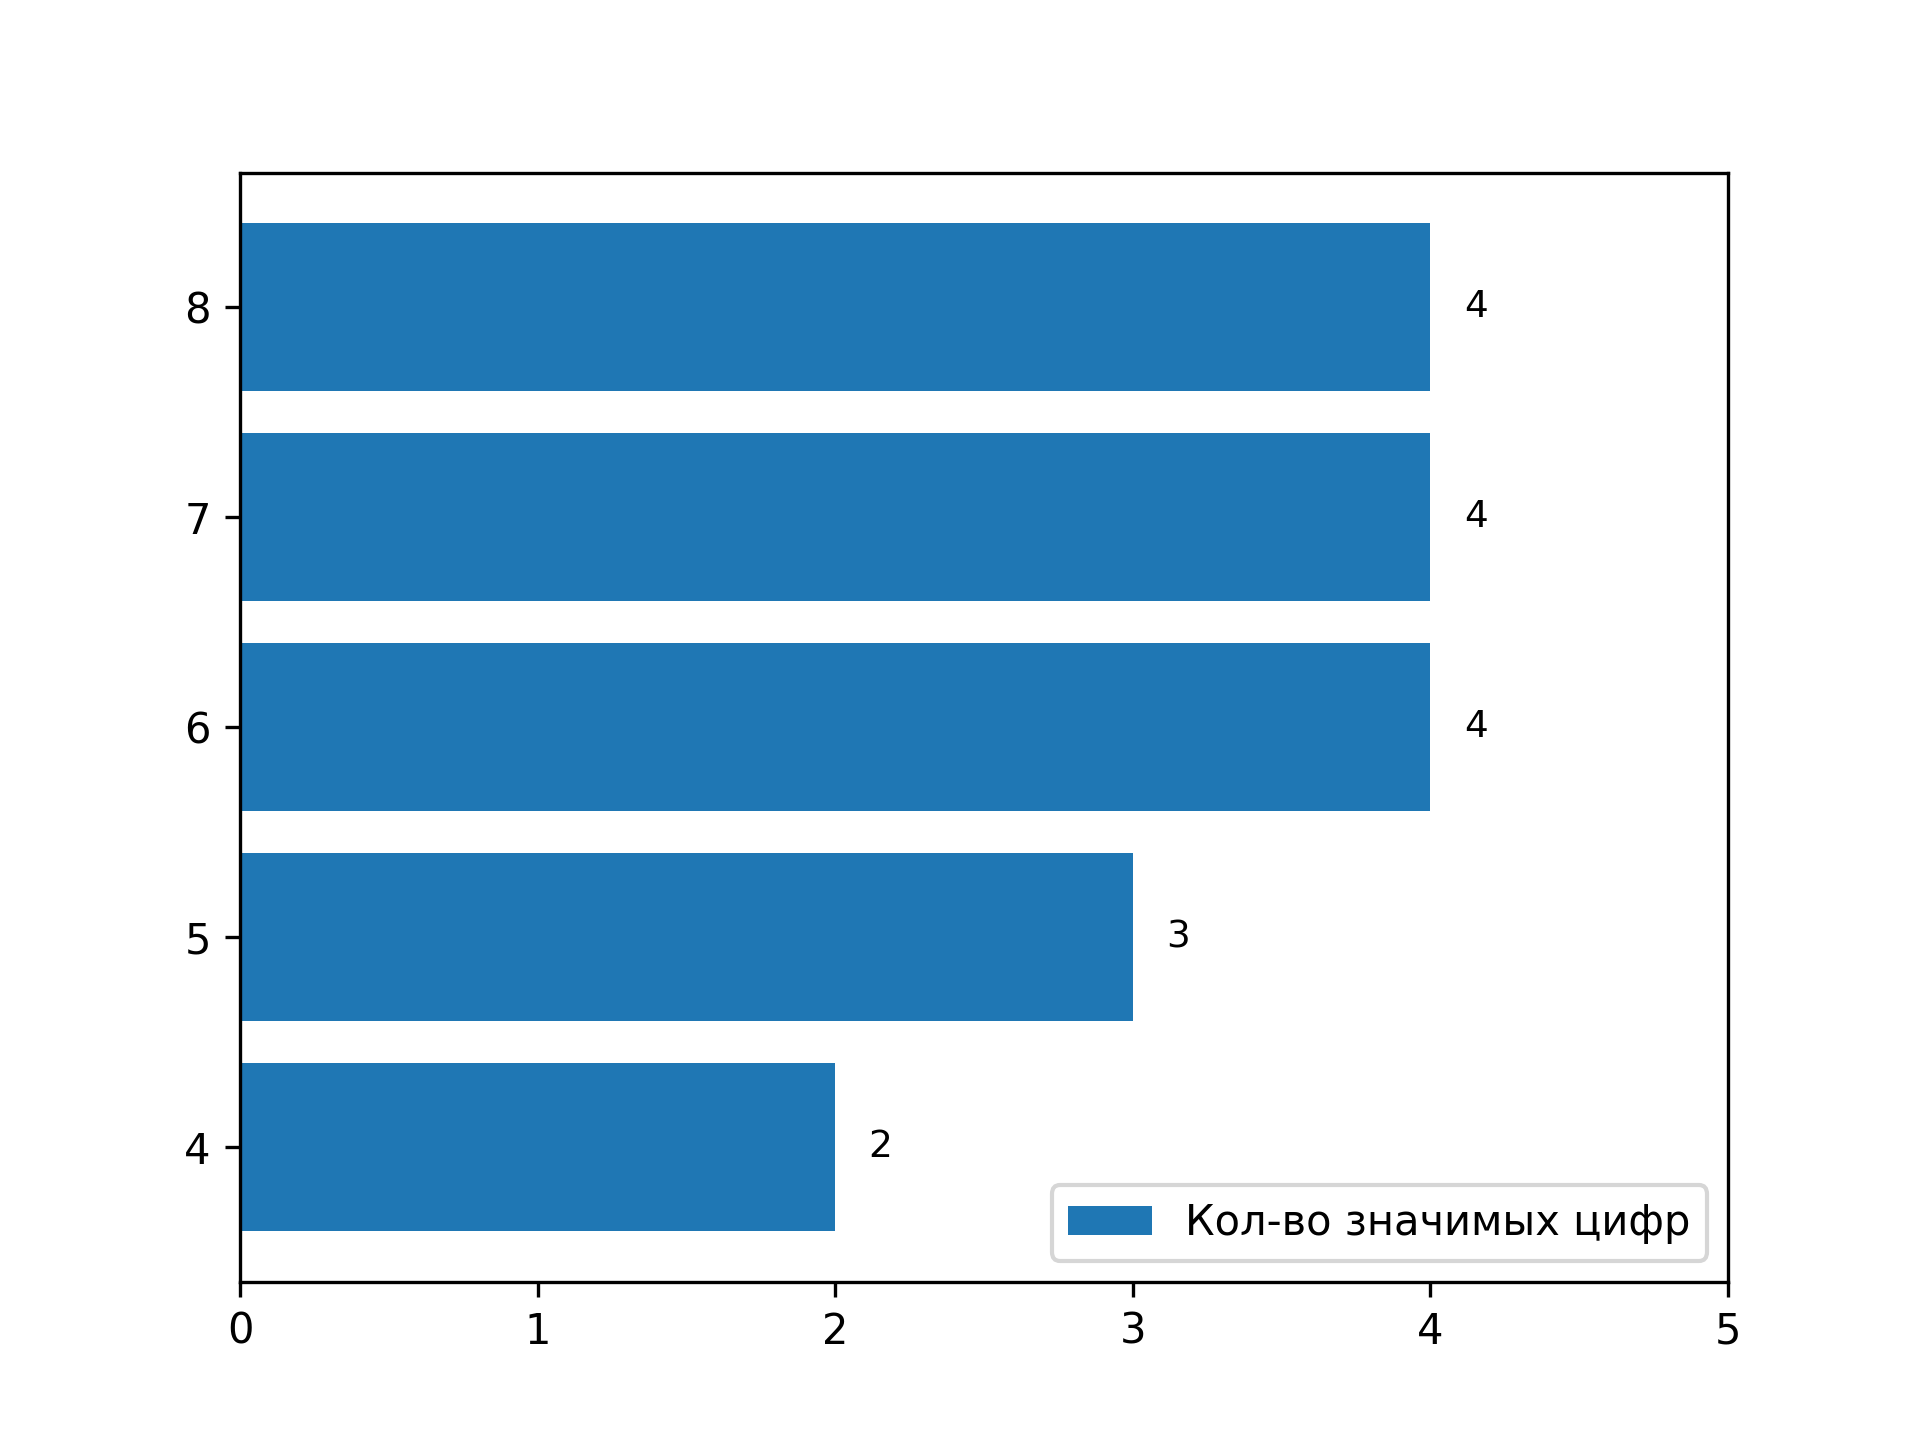
\includegraphics[width=\textwidth]{plots/series_fixed_n_digits.png}
\end{center}

\end{document}